 
\chapter{工具变量方法的应用：模糊回归不连续设计}
 \label{chapter::iv-frdd}



第\ref{chapter::overlap}章介绍的回归不连续设计以及第\ref{chapter::iv-experiment}章至第\ref{chapter::iv-econometric}章介绍的工具变量方法，都是{\it 自然实验}的两个重要范例。这些研究设计与第\ref{part::rcts}章所述的随机对照实验相比虽不够理想，却具备类似随机实验的特征；正因如此它们才被称为自然实验。 


将回归不连续设计与工具变量方法相结合便形成了{\it 模糊回归不连续设计}，这也是一种重要的自然实验形式。本文将先通过实例引入该概念，随后给出其数学表述。  




\section{实例说明}
\label{sec::frdd-motivation}

第\ref{chapter::overlap}章已介绍过回归不连续设计。以下三个实例与其略有区别：在这些实例中，实验处理并非由运行变量直接决定；相反，运行变量会在断点处使个体接受处理的概率发生突变。 

\begin{example}\label{eg::indianroad}
2000年，印度政府启动了“总理乡村道路计划”；至2015年，该计划已为近20万个村庄修建了全天候道路。\citet{asher2020rural}基于村庄级数据，运用回归不连续设计来估算新修道路对各种经济指标的影响。该计划的实施标准参照了2001年人口普查数据，以特定阈值来决定优先资助的村庄规模。若某村庄在统计年份前新建了道路，则视为接受了处理。不过，村庄人口规模与阈值间的差距并不决定处理状态本身，仅在断点0处影响到接受处理的概率。 
\end{example}


\begin{example}\label{eg::italianuniversity}
\citet{li2015evaluating}借助2004至2006年间两所意大利大学新生的数据，评估了助学金对辍学率的因果效应。凡家庭标准化收入低于15,000欧元的申请者均有资格获得资助。为简化分析，我们定义运行变量为15,000减去标准化家庭收入。由于必须先提交申请方能获得资助，因此资格判定与申请行为共同决定了最终处理状态。尽管运行变量同样在断点0处改变了处理概率，但它本身亦不决定处理状态。 
\end{example}



\begin{example}
\citet{amarante2016cash}估计了胎儿在子宫内暴露于一项社会援助计划对出生结局的影响。他们利用乌拉圭{\it Plan de Atención Nacional a la Emergencia Social}计划形成的断点回归。这是一项面向最贫困的百分之十家庭的临时社会援助计划，于2005年4月至2007年12月实施。预测收入评分低于预定阈值的家庭被分配参加该计划。这一评分并不完全决定母亲是否在孕期至少收到一次计划补助，但会改变最终接受处理的概率。出生结局包括出生体重、妊娠周数等。 
\end{example}


上述例子称为模糊断点回归，以区别于第\ref{chapter::overlap}章的精确断点回归。下面将在第\ref{sec::application-frdd}章分析例\ref{eg::indianroad}和例\ref{eg::italianuniversity}中的数据。 

\section{数学表述}
\label{sec::frdd-math}


设 $X_i$ 为运行变量，它决定了
$$
Z_i = I(X_i \geq x_0)
$$
其中 $x_0$ 为预定断点。实际接受的处理 $D_i$ 未必等于 $Z_i$，但条件概率 $\pr(D_i=1\mid X_i = x)$ 会在 $x_0$ 处产生跳变。图\ref{fig::rdd-compare}对比了严格与模糊回归不连续设计下的处理概率分布。其中后者包含一个特例：$\pr(D=1\mid X < x_0) = 0$，此情形恰与例\ref{eg::italianuniversity}相契合。 


\begin{figure}
\centering
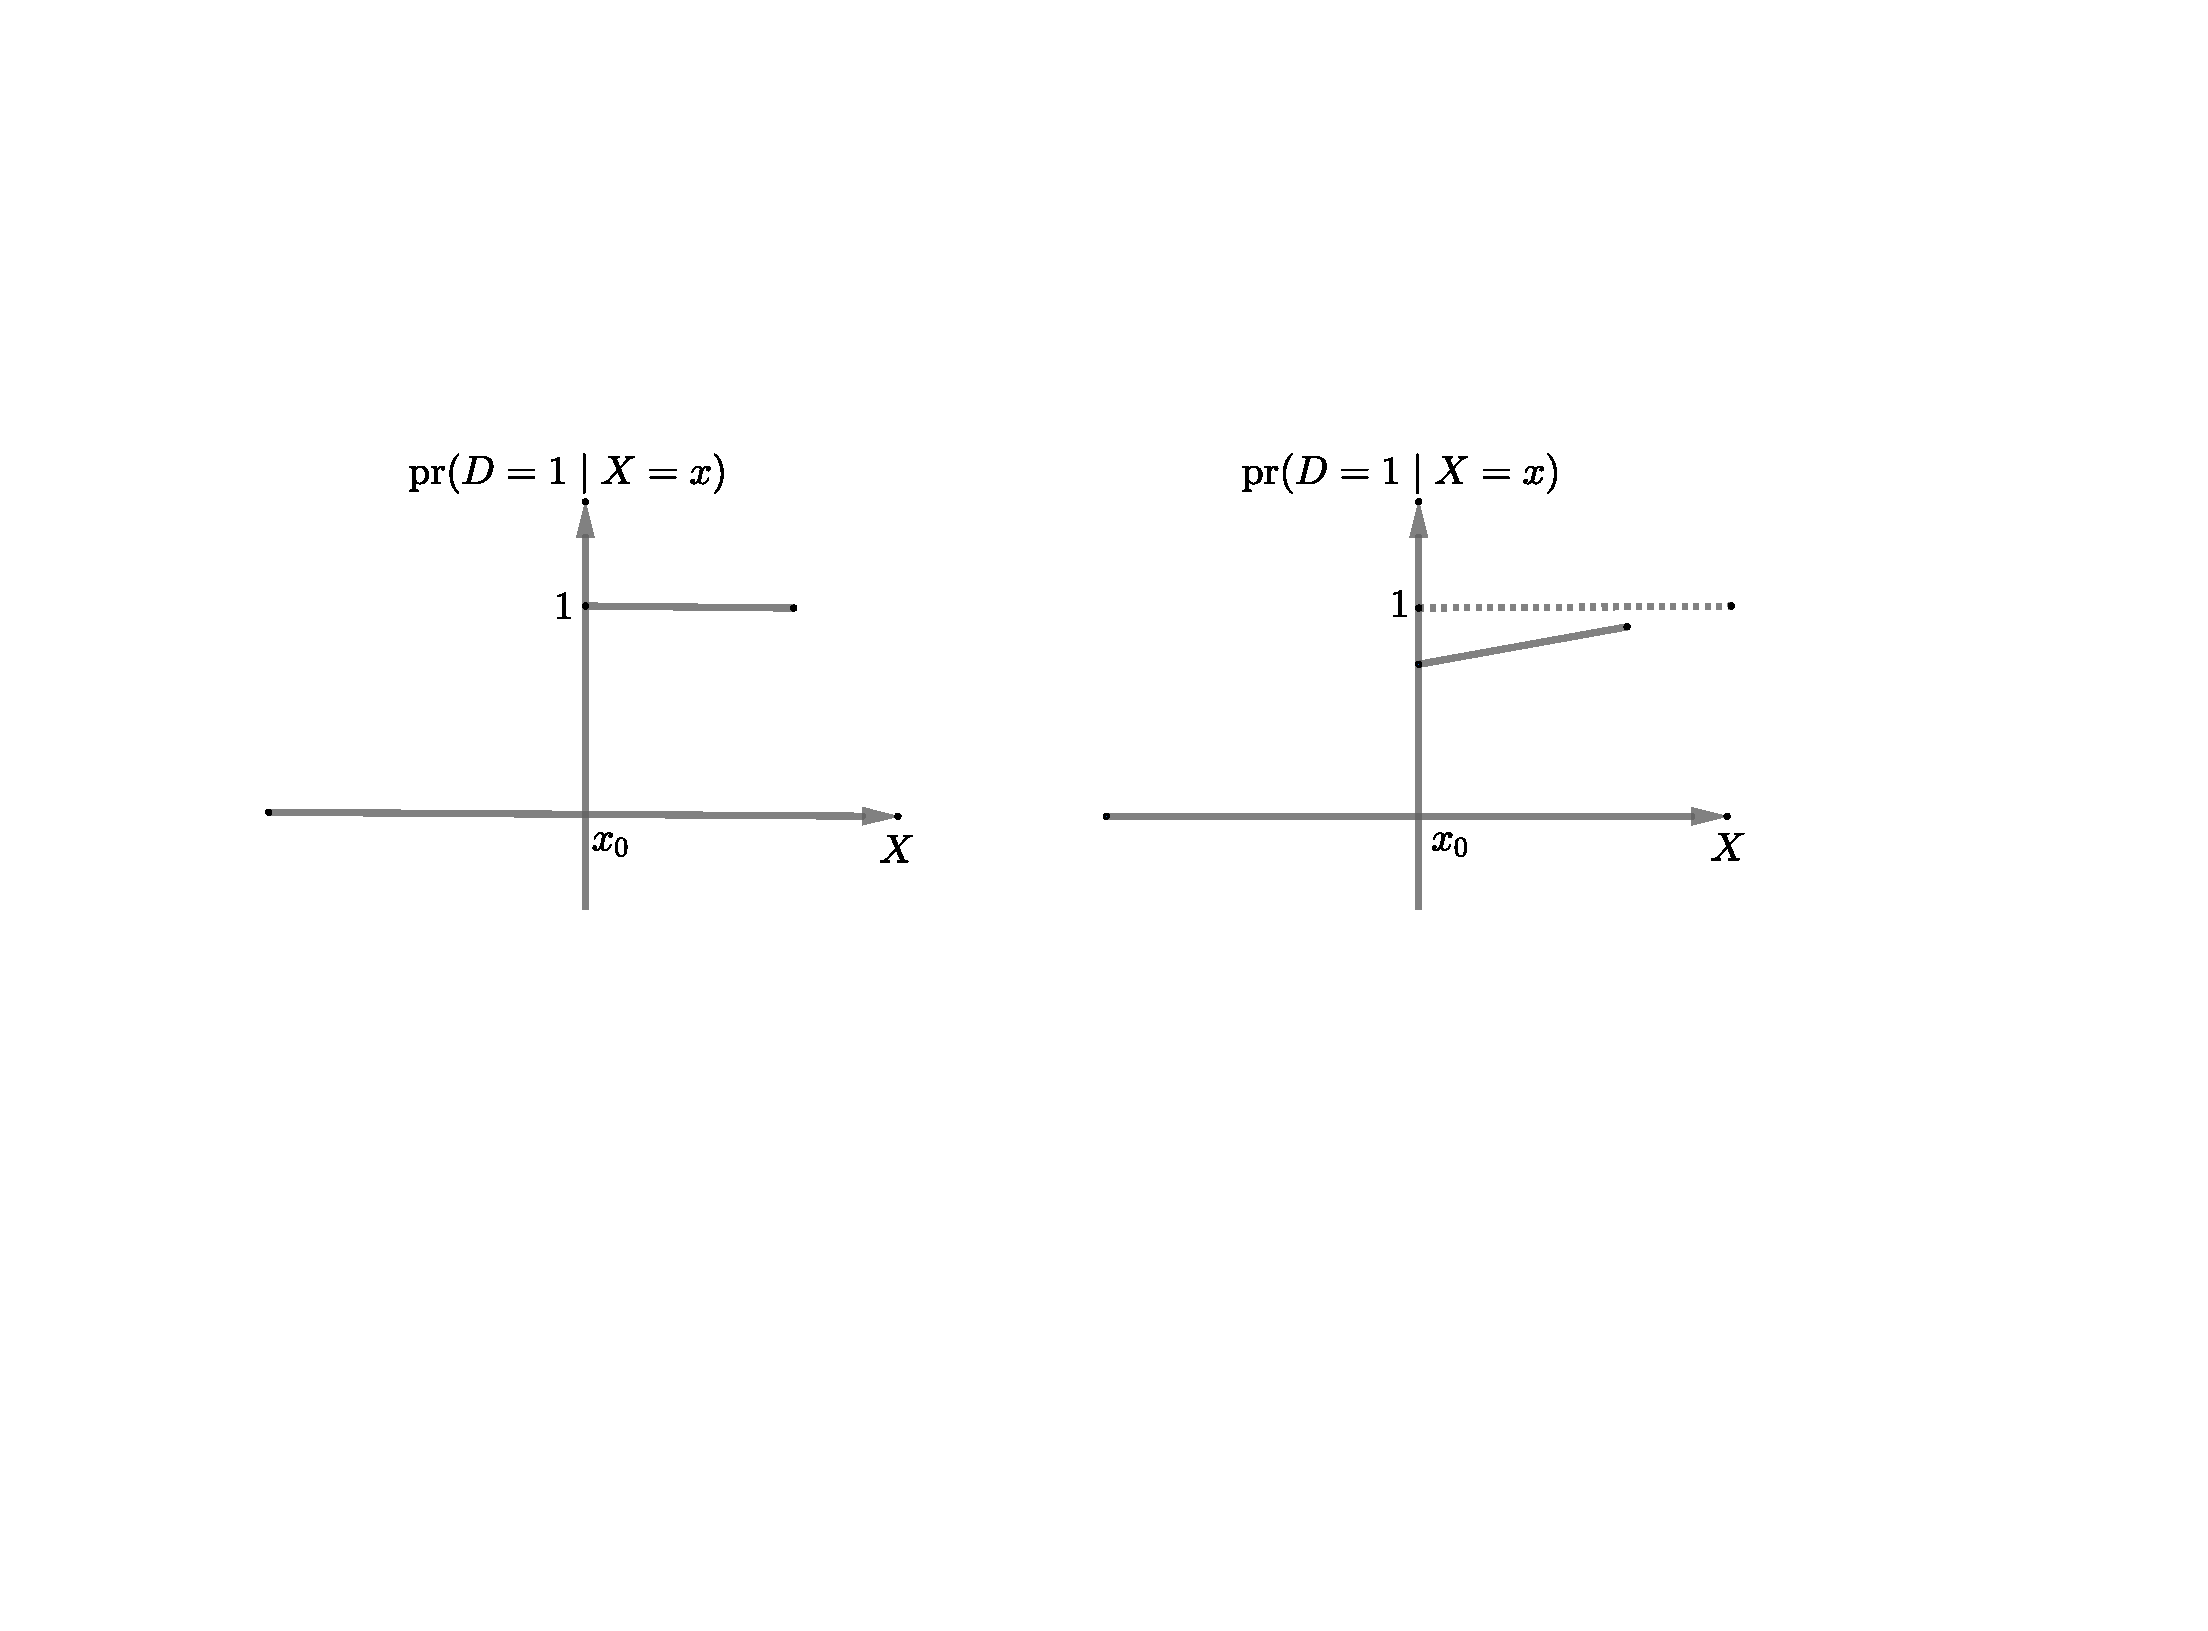
\includegraphics[width = \textwidth]{figures/RDcompare.pdf}
\caption{严格与模糊回归不连续设计的处理分配差异}\label{fig::rdd-compare}
\end{figure}






令$Y_i$为关注的结果。将$Z_i$视为分配的处理，可定义潜在结果$\{ D_i(1), D_i(0), Y_i(1), Y_i(0) \}$。根据定理\ref{thm::identification-rdd}，$Z$的精确断点回归可识别\begin{eqnarray*}
\tau_D(x_0)  &=& E\{ D(1) - D(0)  \mid X=x_0 \}\\
&=& \lim_{\varepsilon \rightarrow 0+} E( D \mid Z=1, X=x_0+\varepsilon ) - \lim_{\varepsilon \rightarrow 0+} E( D \mid Z=0, X=x_0-\varepsilon )
\end{eqnarray*}和\begin{eqnarray*}
\tau_Y(x_0)  &=& E\{ Y(1) - Y(0)  \mid X=x_0 \}\\
&=& \lim_{\varepsilon \rightarrow 0+} E( Y \mid Z=1, X=x_0+\varepsilon ) - \lim_{\varepsilon \rightarrow 0+} E( Y \mid Z=0, X=x_0-\varepsilon )
\end{eqnarray*}以$Z$作为$D$的工具变量，并在$X = x_0$处施加工具变量假设，即可应用定理\ref{thm::CACE-identification}识别局部依从者平均因果效应。

\begin{theorem}
\label{thm::identification-frdd}
假设处理由$Z = I(X \geq x_0)$决定，其中$x_0$为预定阈值。在$x_0$的无穷小邻域内，假设单调性$$
D_i(1) \geq D_i(0)
$$和排除限制$$
D_i(1) = D_i(0) \Longrightarrow  Y_i(1) = Y_i(0) 
$$成立。局部依从者平均因果效应定义为$$
 \tau_\cp(x_0)   
= E\{ Y(1) - Y(0)  \mid D(1)  >  D(0),  X=x_0 \},
$$可以由$$
 \tau_\cp(x_0)   
=  \frac{ E\{ Y(1) - Y(0)  \mid X=x_0 \}  }{E\{ D(1) - D(0)  \mid X=x_0 \}} .
$$识别。进一步假设$E\{ D(1) \mid X=x   \}$和$E\{ Y(1) \mid X=x   \}$在$x=x_0$处右连续，$E\{ D(0) \mid X=x   \}$和$E\{ Y(0) \mid X=x   \}$在$x=x_0$处左连续。若$E(D\mid X=x)$在$x=x_0$处存在非零跳跃，则局部依从者平均因果效应可以由$$
 \tau_\cp(x_0) 
 = \frac{ \lim_{\varepsilon \rightarrow 0+} E( Y \mid Z=1, X=x_0+\varepsilon ) - \lim_{\varepsilon \rightarrow 0+} E( Y \mid Z=0, X=x_0-\varepsilon ) }
{\lim_{\varepsilon \rightarrow 0+} E( D \mid Z=1, X=x_0+\varepsilon ) - \lim_{\varepsilon \rightarrow 0+} E( D \mid Z=0, X=x_0-\varepsilon )}
$$识别。 
\end{theorem}


 定理\ref{thm::identification-frdd}实为定理\ref{thm::identification-rdd}与\ref{thm::CACE-identification}的综合形式。其证明过程留作习题\ref{para::proof-theorem-frd}。 
 

无论严格抑或模糊回归不连续设计，选取断点邻域范围均属核心操作。一般而言，较小邻域能降低偏差却增加方差；较大邻域则反之。这种偏差-方差权衡亟需通过敏感性分析加以权衡。当前已有基于统计判据的自动选择方法，却需满足若干严苛前提条件。因此就实际分析而言，多步调整邻域范围并开展敏感性检验方为稳妥策略。 

假设已用带宽$h$确定$x_0$的邻域。对于满足$X_i \in [x_0-h, x_0 + h]$的数据，可用$$
\hat{\tau}_D(x_0) = \text{the coefficient of } Z_i
\text{ in the OLS fit of } D_i \text{ on } \{1, Z_i, R_i, L_i\},
$$估计$\tau_D(x_0) $，用$$
\hat{\tau}_Y(x_0) = \text{the coefficient of } Z_i
\text{ in the OLS fit of } Y_i \text{ on } \{1, Z_i, R_i, L_i\},
$$估计$\tau_Y(x_0) $，其中回顾定义$R_i = \max(X_i - x_0, 0)$和$L_i= \min (X_i - x_0, 0)$。于是局部依从者平均因果效应可估计为$$
\hat\tau_\cp(x_0)  = \hat{\tau}_Y(x_0) / \hat{\tau}_D(x_0).
$$这是间接最小二乘估计量。由定理\ref{thm::ils=2sls}，它在数值上等于$$
\text{the coefficient of } D_i
\text{ in the TSLS fit of } Y_i \text{ on } \{1, D_i, R_i, L_i\}  
$$其中用$Z_i$作为$D_i$的工具变量。总之，选定$h$后，$ \tau_\cp(x_0)$的估计就归结为对阈值附近的局部数据实施两阶段最小二乘。  


\section{应用示例}
 \label{sec::application-frdd}

\subsection{再分析 \citet{asher2020rural} 的数据}
\label{sec::indian-road-data}

重新考察例\ref{eg::indianroad}。对于一系列$h$，可使用结果变量\ri{occupation_index_andrsn}计算点估计和标准误。 
\begin{lstlisting}
library("car")
road_dat = read.csv("indianroad.csv")
table(road_dat$t, road_dat$r2012)
road_dat$runv = road_dat$left + road_dat$right
## sensitivity analysis 
seq.h  = seq(10, 80, 1)
frd_sa = lapply(seq.h, function(h){
  road_sub = subset(road_dat, abs(runv)<=h)
  road_sub$r2012hat = lm(r2012 ~ t + left + right,
                         data = road_sub)$fitted.values
  tslsreg = lm(occupation_index_andrsn ~ r2012hat + left + right,
               data = road_sub)
  res = with(road_sub,
             {
               occupation_index_andrsn -
                 cbind(1, r2012, left, right)%*%coef(tslsreg)
             })
  tslsreg$residuals = as.vector(res)
  
  c(coef(tslsreg)[2],
    sqrt(hccm(tslsreg, type = "hc2")[2, 2]),
    length(res))
})
frd_sa = do.call(rbind, frd_sa)
\end{lstlisting}
图\ref{fig::indian_road}呈现了分析结果：仅当 $h$ 取值较大时才出现显著处理效应。 

\begin{figure}
\centering
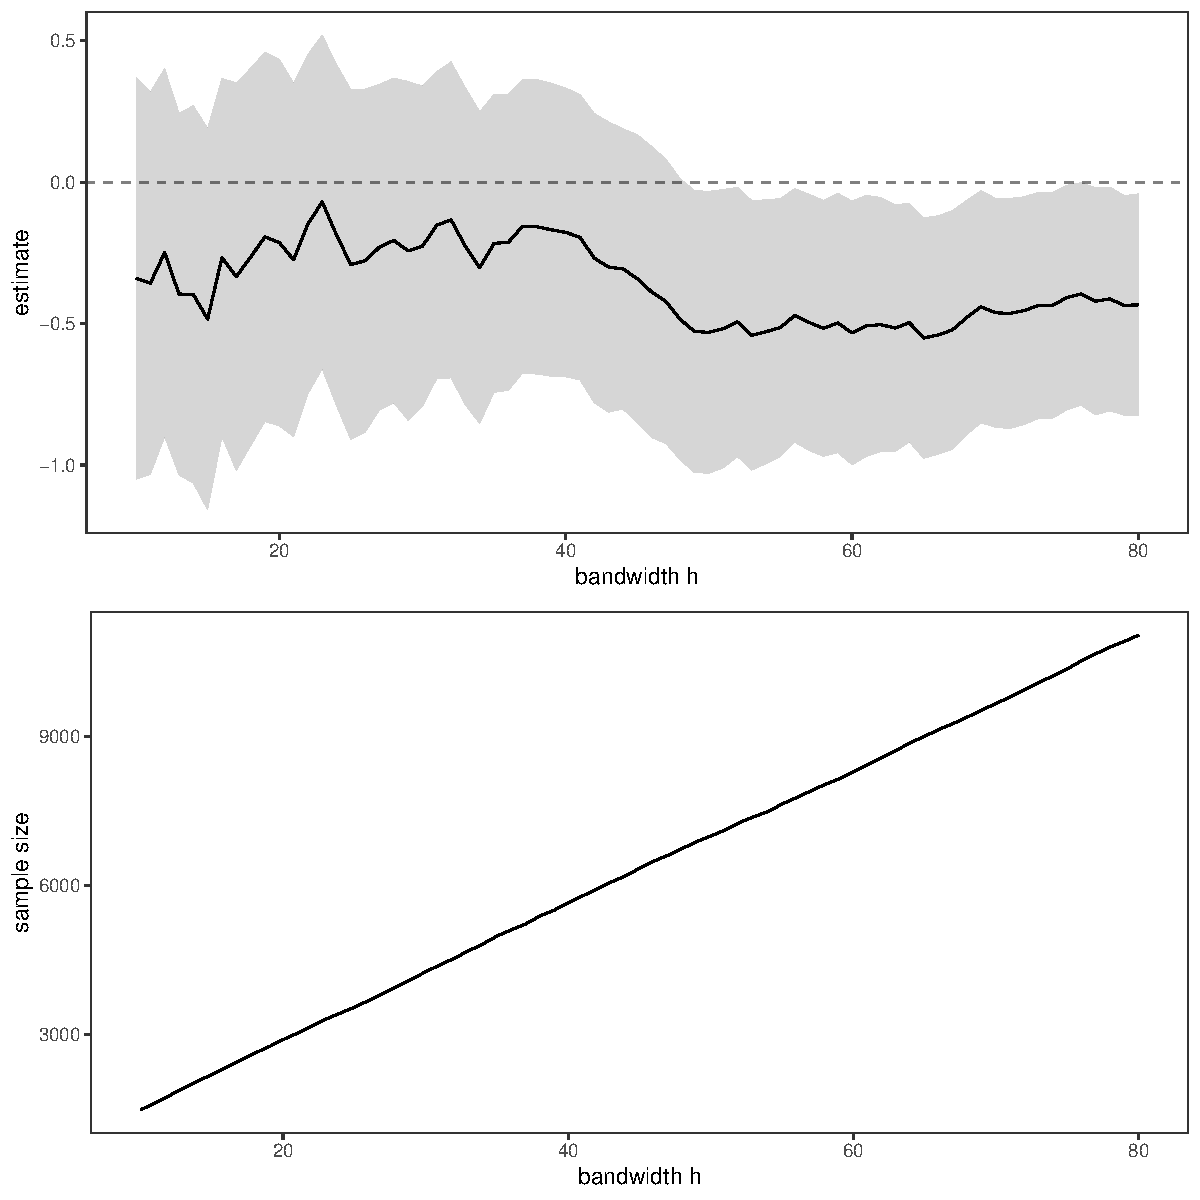
\includegraphics[width = 0.9\textwidth]{figures/frd_indian.pdf}
\caption{基于两步法再分析\citet{asher2020rural}数据所得点估计与标准误}
\label{fig::indian_road}
\end{figure} 


\ri{rdrobust}包可自动确定最优带宽。分析结果显示新建道路并未对目标指标产生明显影响。 

\begin{lstlisting}
> library("rdrobust")
> frd_road = with(road_dat,
+                 {
+                   rdrobust(y = occupation_index_andrsn,
+                            x = runv,
+                            c = 0,
+                            fuzzy = r2012)
+                 })
> res = cbind(frd_road$coef, frd_road$se)
> round(res, 3)
                Coeff Std. Err.
Conventional   -0.253     0.301
Bias-Corrected -0.283     0.301
Robust         -0.283     0.359
\end{lstlisting}

\subsection{再分析 \citet{li2015evaluating} 的数据}
 \label{sec::italian-university}
 
 
 重新考察例\ref{eg::italianuniversity}。运行变量为15,000减去标准化收入。在分析中，将数据限制为运行变量位于$[-5,000,5,000]$内的子集，再将运行变量除以$5,000$，使其取值限制于$[-1,1]$，阈值为零。下面计算一系列$h$对应的点估计和标准误。 
\begin{lstlisting}
library("car")
italy = read.csv("italy.csv")
italy$left  = pmin(italy$rv0, 0)
italy$right = pmax(italy$rv0, 0)
## sensitivity analysis 
seq.h  = seq(0.1, 1, 0.01)
frd_sa = lapply(seq.h, function(h){
  italy_sub = subset(italy, abs(rv0)<=h)
  italy_sub$Dhat = lm(D ~ Z + left + right,
                      data = italy_sub)$fitted.values
  tslsreg = lm(outcome ~ Dhat + left + right,
               data = italy_sub)
  res = with(italy_sub,
             {
               outcome -
                 cbind(1, D, left, right)%*%coef(tslsreg)
             })
  tslsreg$residuals = as.vector(res)
  
  c(coef(tslsreg)[2],
    sqrt(hccm(tslsreg, type = "hc2")[2, 2]),
    length(res))
})
frd_sa = do.call(rbind, frd_sa)
 \end{lstlisting}
 


  图\ref{fig::italy_university}显示测算数据：无论何种带宽设置，助学金对辍学率均无明显效应。 
\begin{figure}
\centering
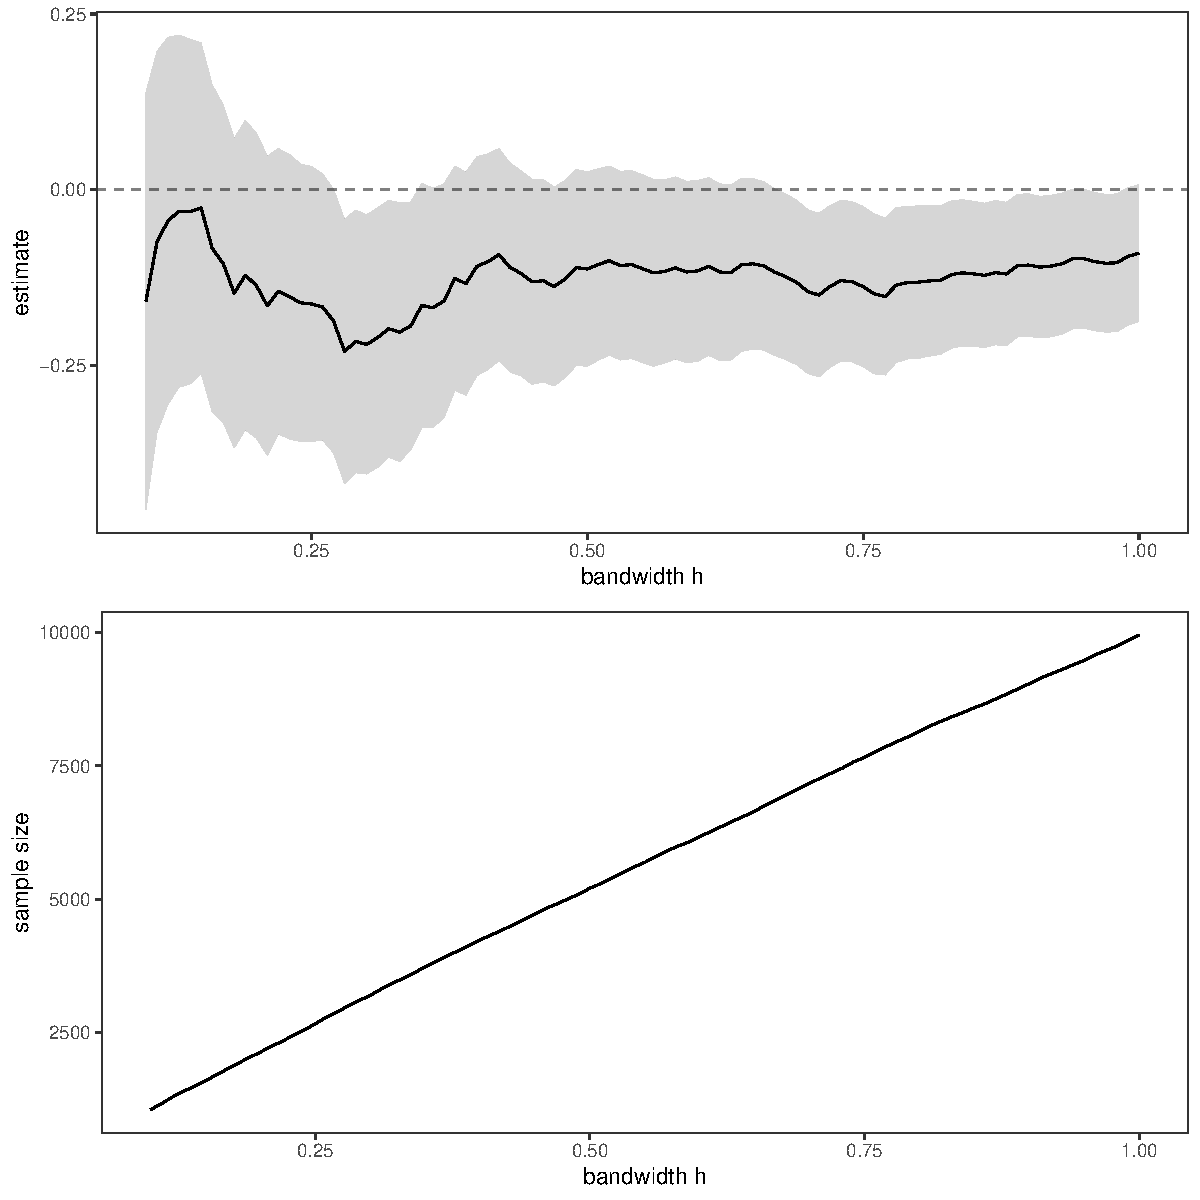
\includegraphics[width = 0.9\textwidth]{figures/frd_italy.pdf}
\caption{基于两步法再分析\citet{li2015evaluating}数据所得点估计及标准误}
\label{fig::italy_university}
\end{figure} 
 
 
 
使用\ri{rdrobust}包得到的结果也支持相同结论。 
 
 \begin{lstlisting}
> library("rdrobust")
> frd_italy = with(italy,
+                  {
+                    rdrobust(y = outcome,
+                             x = rv0,
+                             c = 0,
+                             fuzzy = D)
+                  })
> res = cbind(frd_italy$coef, frd_italy$se)
> round(res, 3)
                Coeff Std. Err.
Conventional   -0.149     0.101
Bias-Corrected -0.155     0.101
Robust         -0.155     0.121
 \end{lstlisting}
 
 
 
 \section{讨论}


第\ref{chapter::overlap}章与本章均基于运行变量条件下潜在结果期望值的连续性来构建回归不连续分析框架。此视角虽具数学简洁性，却仅能在断点处精确估计局部效应。\citet{hahn2001identification}开拓了这一研究方向。 

另一种较少采用的视角基于{\it 局部随机化}\citep{cattaneo2015randomization, li2015evaluating}。若将运行变量看作某个潜在真实量的含噪测量，且阈值的选取带有一定任意性，则阈值附近的单位不存在系统差异。这提示，在阈值的小邻域内，各单位像随机实验中一样随机接受处理或对照。类似于第一种视角中选择$h$的问题，这里关键在于确定断点附近多大的范围可以视为随机实验。将这种直觉用数学量化并不容易，因此，在第二种视角下，对一系列$h$开展敏感性分析同样是合理的做法。  


关于回归不连续设计的概念探讨可参考\citet{sekhon2017interpreting}。 



 
\section{作业习题}

\paragraph{定理 \ref{thm::identification-frdd} 的证明}\label{para::proof-theorem-frd}

试证明定理\ref{thm::identification-frdd}。 


\paragraph{数据分析}
 
前文\ref{sec::indian-road-data}已针对指标\ri{occupation_index_andrsn}做了分析。其他相关指标包括\ri{transport_index_andrsn}、\ri{firms_index_andrsn}、\ri{consumption_index_andrsn}与\ri{agriculture_index_andrsn}；它们的物理意义均见原研究文献。请同样测算各变量所受影响程度。 

 

\paragraph{关于\citet{li2015evaluating}分析思路的思考}
\label{problem::italy-srd}

\citet{li2015evaluating}的研究中关键变量为二值申请状态 $A$，其对应潜在结果 $A(1)$ 与 $A(0)$ 分别对应于处理组 $Z=1$ 与对照组 $Z=0$。依定义：
$$
D(1) = A(1), \quad D(0) = 0,
$$
因此符合“顺从者”条件的个体 $\{ D(1), D(0) \} = (1,0)$ 等价于 $A(1) = 1$。这意味着
$$
\tau_\cp(x_0) = E\{ Y(1) - Y(0) \mid A(1) = 1, X = x_0 \}. 
$$
例\ref{sec::italian-university}中分析采用全部样本测定 $\tau_\cp(x_0)$。 

另一种分析是只使用满足$A=1$的单位。此时处理状态由$X$决定，但这种分析可能存在问题，因为\begin{eqnarray}
&& \lim_{\varepsilon \rightarrow 0+} E\{ Y \mid A  = 1, X = x_0 + \varepsilon \} -\lim_{\varepsilon \rightarrow 0+}  E\{ Y \mid A  = 1, X = x_0- \varepsilon  \}  \nonumber  \\
&=& E\{ Y(1) \mid A(1)  = 1,   X = x_0   \} -  E\{ Y(0) \mid A(0)  = 1,   X = x_0   \} .\label{hw::frdd-florence-A=1}
\end{eqnarray}证明\eqref{hw::frdd-florence-A=1}，并解释这种分析为何可能有问题。


说明：\eqref{hw::frdd-florence-A=1}左端是在$A=1$条件下、$X=x_0$处局部平均处理效应的识别公式。\eqref{hw::frdd-florence-A=1}右端则分别是满足$(A(1)  = 1,   X = x_0 )$和$(A(0)  = 1,   X = x_0)$的两个子组的潜在结果均值之差。相关讨论见后面的第\ref{chapter::principal-stratification}章。 
 


 
 \paragraph{推荐阅读}

\citet{imbens2008regression}以潜在结果视角提供了实用分析指引；\citet{lee2010regression}则综述了回归不连续设计在经济学中的应用发展。 
